\chapter{Rekursion}

\section{Lösungsvorschlag}

Der Methode \code{recursion} wird ein ganzzahliger Wert übergeben.\\
Die Methode ruft sich dann $2$-mal mit dem Übergabeparameter $n - 1$ selber auf.\\
Der Rückgabewert der Methodenaufrufe wird addiert, die Summe zurückgegeben:

\begin{minted}[mathescape,
    linenos,
    numbersep=5pt,
    gobble=2]{java}
    return recursion(n - 1) + recursion(n - 1);
\end{minted}\\

\noindent
Die \textit{Abbruchbedingung} ist $n \leq 0$ - in dem Fall liefert die Methode ohne weiteren rekursiven Aufruf den Wert $1$ zurück.\\


\noindent
Für die Rekursionsgleichung $R$ ergibt sich demnach in Abhängigkeit des Eingabewertes $n$ mit $n \in \mathbb{N}$

\begin{equation}
    R(n) = \begin{cases}
               1\ falls\ n\ = 0 \\
               R(n-1) + R(n-1)
    \end{cases}
\end{equation}\\

\noindent
Wie in Abbildung~\ref{fig:recursion} ersichtlich ist, verdoppeln sich die Anrufe für \code{recursion} mit jedem Rekursionsschritt.\\

\begin{figure}
    \begin{center}
        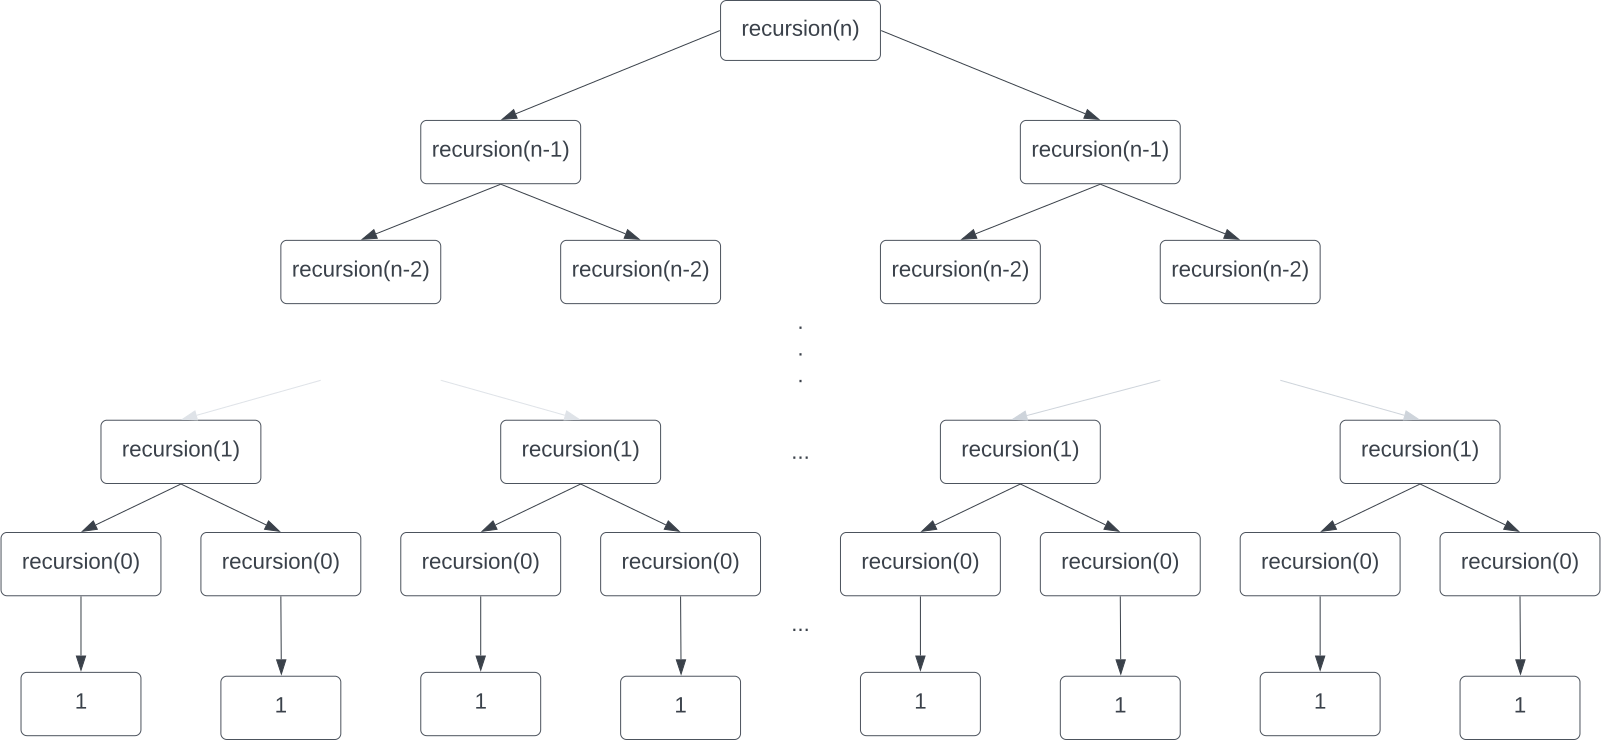
\includegraphics[scale=0.3]{chapters/9. Rekursion/img/recursion}
        \caption{Der Rekursionsbaum der Methode \textit{recursion} (Quelle: eigene)}
        \label{fig:recursion}
    \end{center}
\end{figure}


\noindent
Der initiale Aufruf \code{recursion(n)} ruft $2$-mal \code{recursion(n-1)} auf.\\
Danach wird für jeden dieser Aufrufe \code{recursion(n-2)} aufgerufen, also insg. $4$-mal\ldots bis die Abbruchbedingung $n \leq 0$ erüllt ist.\\
Für die Anzahl $m$ der Aufrufe von \code{recursion} ergibt sich somit


\begin{equation}
     m = 1 + 2 + 4 + \dots + 2^n = \sum_{i=0}^n 2^i
    \label{eq:reccalls}
\end{equation}\\

\noindent
Für den Rekursionsbaum ist der Rückgabewert bei Erfüllung der Abbruchbedingung von Interesse, der den Hinweis zu dem Ergebnis in Abhängigkeit von $n$ liefert.\\
Die Anzahl der Blätter des Baumes entsprechen dem letzten Summanden der Gleichung \ref{eq:reccalls}, mit $i=n$
also $2^n$.\\
Da letztendlich deren Summe das Ergebnis der Methode \code{recursion} liefert, ist das gesuchte Ergebnis $2^n$.\\

\noindent
Die Rekursionstiefe des Baumes entspricht $n$, wobei sich auf jeder Ebene die Anzahl der rekursiven Aufrufe verdoppelt\footnote{
    Anzahl gleichzeitig aktiver \textit{rekursiver} Aufrufe; der erste Aufruf wird i.d.R. nicht dazugezählt und entspricht der ``Wurzel`` des Rekursionsbaums.
    Die Rekursionstiefe entspricht damit der \textit{Höhe} des Baumes (vgl. Skript (Teil 2) S.34); bzgl. der Begriffsbestimmung siehe hierzu auch \cite[144 f.]{CK75}.
}.\\
Mit der Anzahl der Rekursionsaufrufe lässt sich auch auf die Komplexitätsklasse schliessen, die mit $O(2^n)$ \textbf{exponentiell} ist.

